\section{How can I contribute to a project?}

\begin{frame}[fragile,allowframebreaks]{Short answer}

    \begin{figure}
    \centering
    \subfigure{
\includegraphics[width=0.24\textwidth]{assets/GitHub_Logo.png}}\hspace{0.02\textwidth}
    \subfigure{
\includegraphics[width=0.24\textwidth]{assets/Git-Logo-1788C.png}}\hspace{0.02\textwidth}
    \subfigure{
\includegraphics[width=0.26\textwidth]{assets/gitlab-logo-200.png}}
    
    \label{fig:SftwToContribute}
    \end{figure}

\end{frame}

\automateframe{A quick example}{
\begin{itemize}
    \item Suppose you want to \textbf{contribute} to a project which is currently working fine
    \item And you want to make a change \textbf{without breaking anything}...
\end{itemize}
}

\begin{frame}{A quick example}
\begin{itemize}
    \item You could use some Cloud Based service and copy your folder and files
\end{itemize}

\begin{figure}
    \centering
    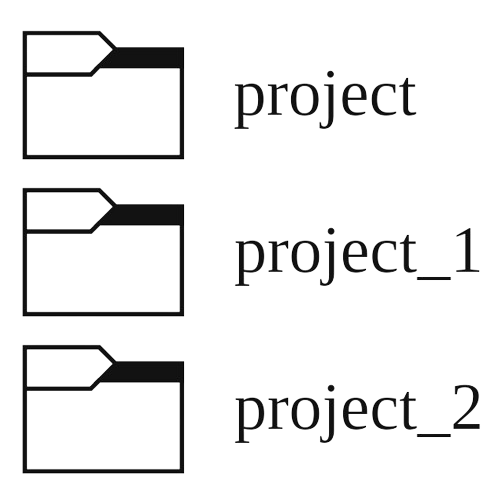
\includegraphics[width=0.35\linewidth]{assets/dir_chaos.png}
    \label{fig:dir_chaos}
\end{figure}

\end{frame}

\begin{frame}{A quick example}
\begin{itemize}
    \item And find yourself with a real mess...
\end{itemize}

\begin{figure}
    \centering
    
\includegraphics[width=0.35\linewidth]{assets/pure_chaos_nobg.png}
    \label{fig:pure_chaos}
\end{figure}

\end{frame}


